\documentclass{beamer}
%\usepackage{beamerarticle}
\usepackage{heppennames}
\usepackage{hepnicenames}
\usepackage{graphicx} 
\usepackage{multirow}
\usepackage{amsbsy,amsmath,amssymb}
\usepackage{booktabs}
% ********** Styl prezentacji **********
\mode<presentation>
{
	\usetheme{Singapore}
  \setbeamercovered{transparent}
   \setbeamertemplate{footline}[frame number] 
%   \setbeamertemplate{navigation symbols}{ 
%   \insertslidenavigationsymbol
%   \insertframenavigationsymbol
%   \insertsubsectionnavigationsymbol
%   \insertsectionnavigationsymbol
%   \insertdocnavigationsymbol
%   \insertbackfindforwardnavigationsymbol
%   \hskip 0.3cm
%   %\insertframenumber / \inserttotalframenumber  % <<< frame #
%   %\insertpagenumber / \insertpresentationendpage % <<< page #
% } 
}

\usepackage[english]{babel}
\usepackage[latin1]{inputenc}

% font definitions, try \usepackage{ae} instead of the following
% three lines if you don't like this look
\usepackage{mathptmx}
\usepackage[scaled=.90]{helvet}
\usepackage{courier}


\usepackage[T1]{fontenc}

\author{S. Poss for the CERN LCD group}
\institute[CERN]{CERN}

\subject{CLICCDR}
\AtBeginSection[]
{   
{
    \usebackgroundtemplate{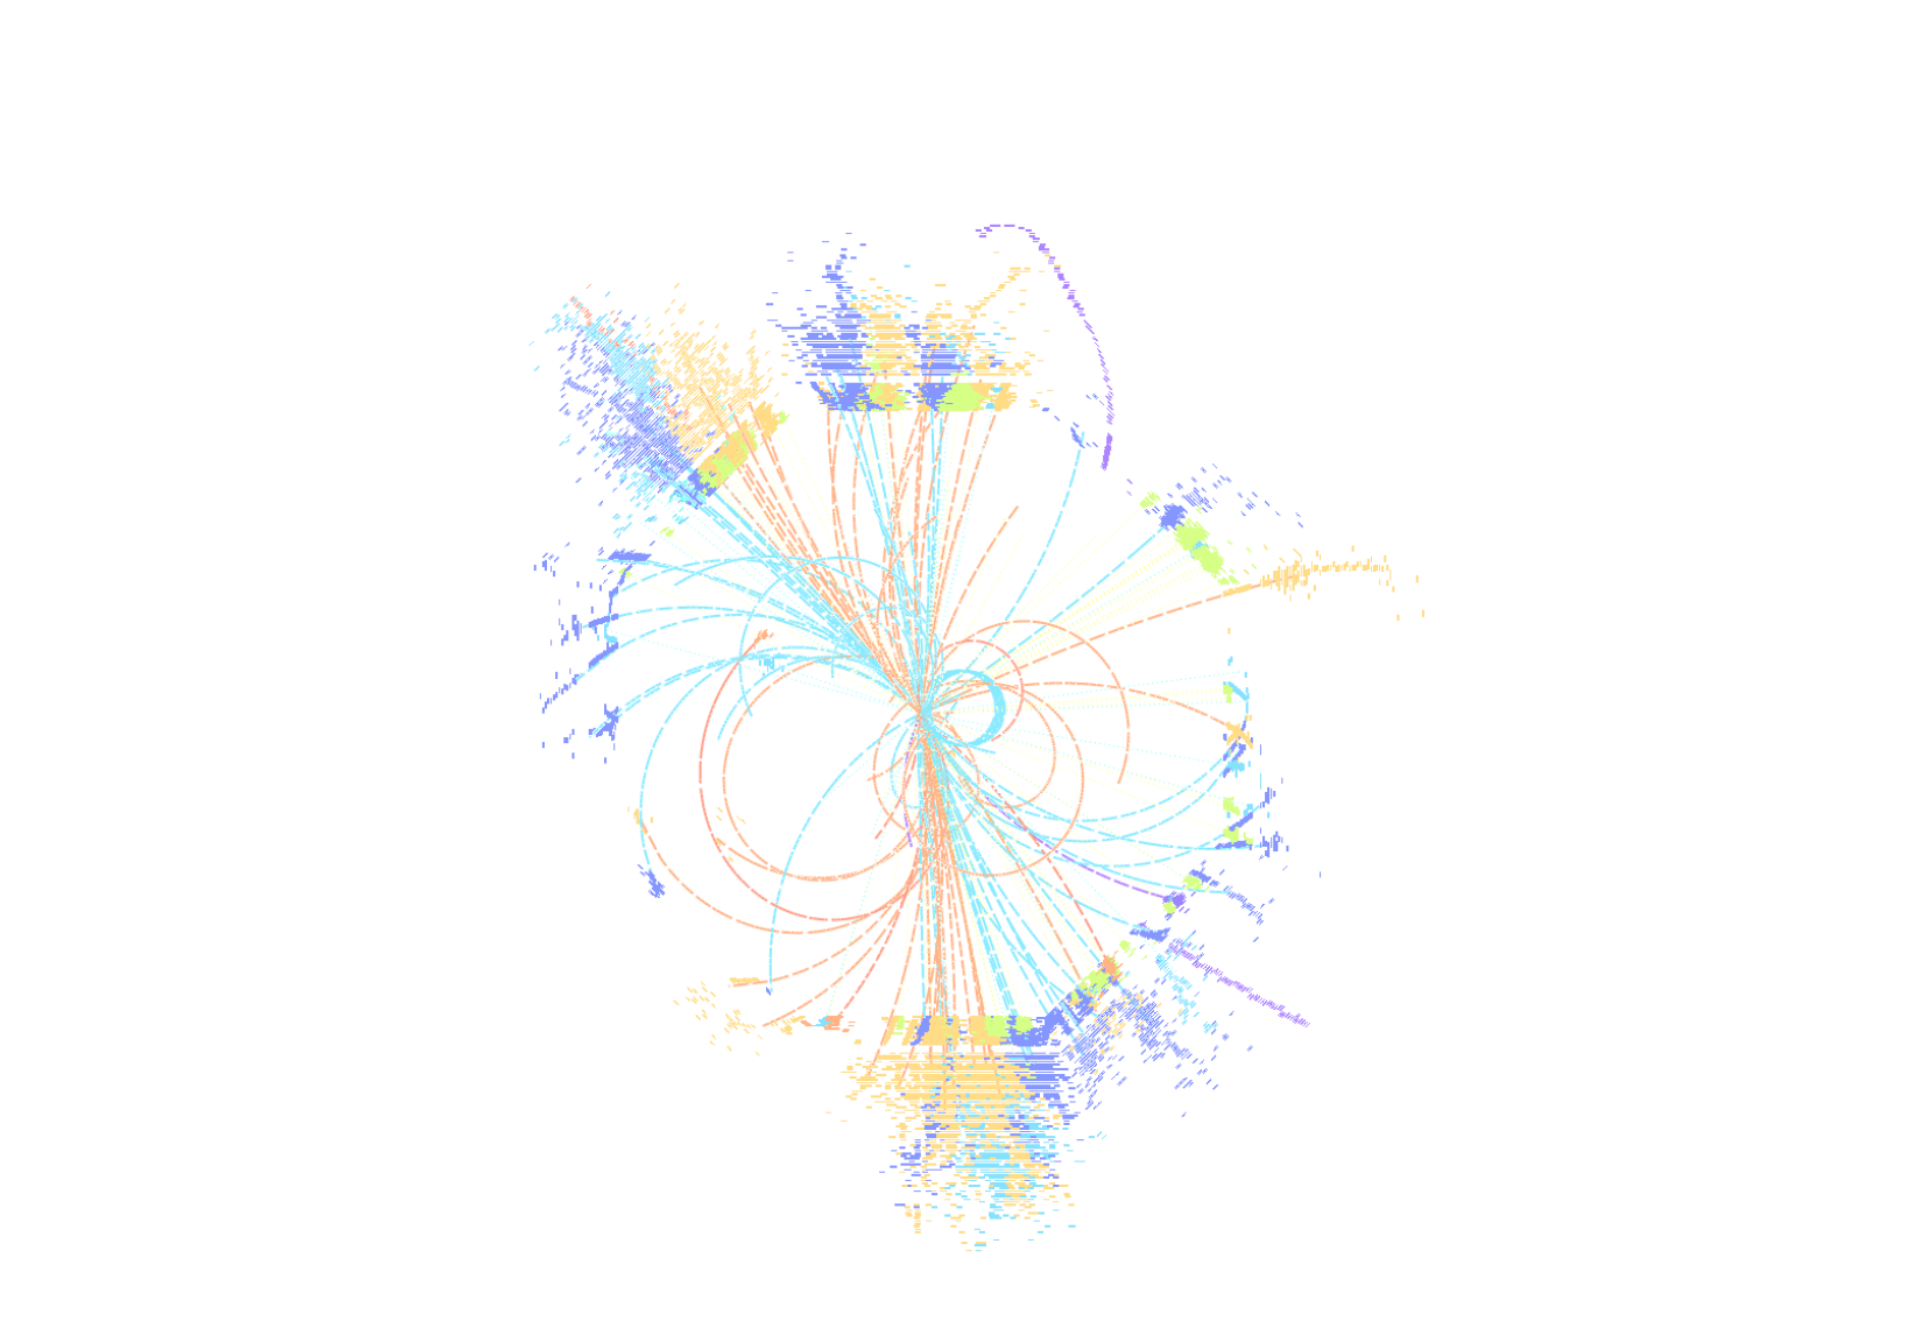
\includegraphics[width=\paperwidth]{background.png}}
	\begin{frame}<beamer>
		\frametitle{Outline}
		\tableofcontents[currentsection,currentsubsection]
	\end{frame}
}
}
\title[]{CLIC Physics and detectors CDR}
%%\subtitle{Our experience}

\date{\today}

\begin{document}

{
\usebackgroundtemplate{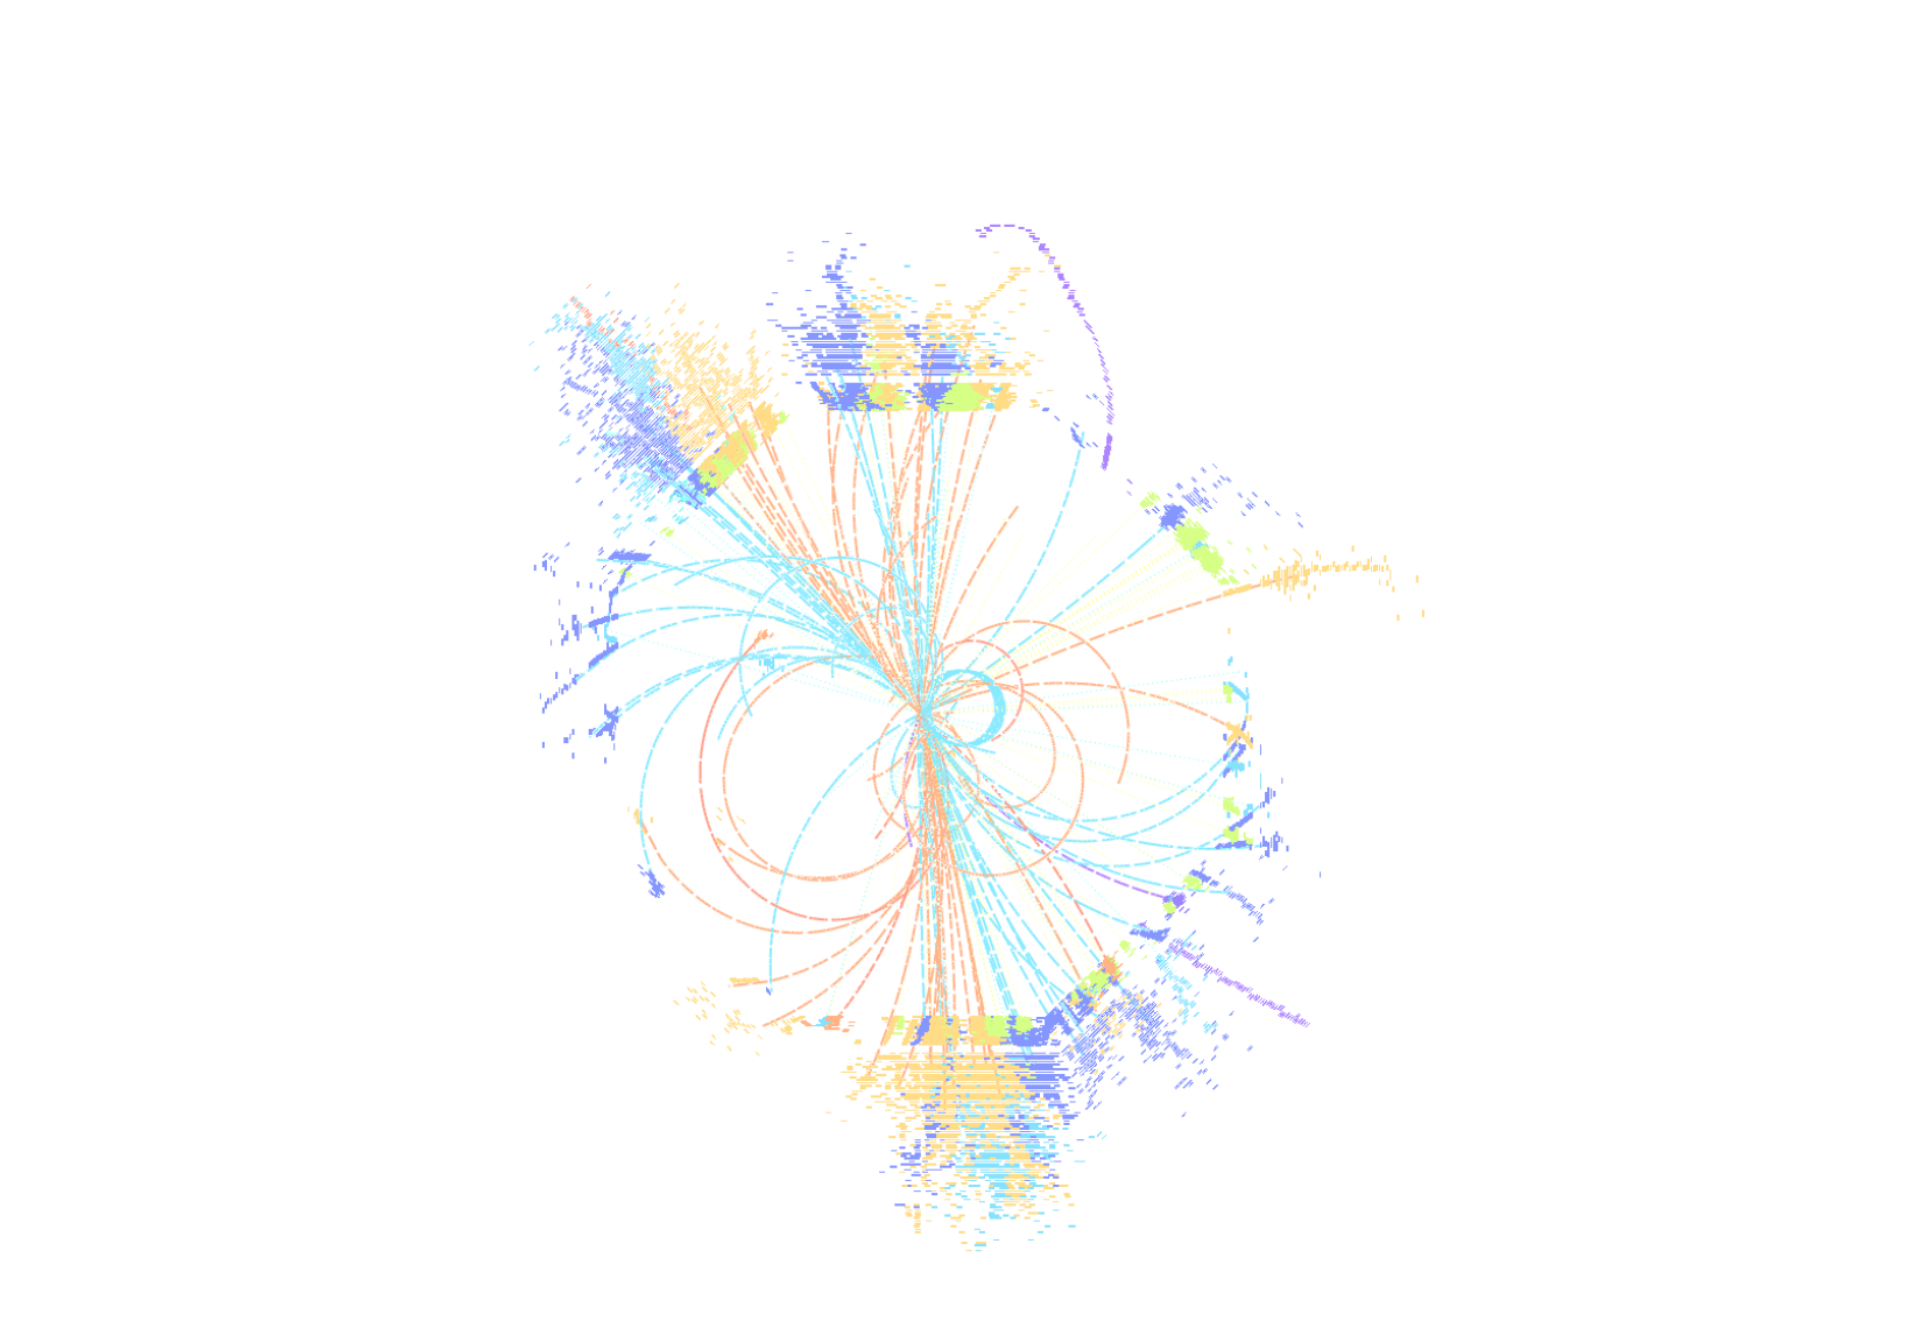
\includegraphics[width=\paperwidth]{background.png}}

\begin{frame}
	\titlepage
\end{frame}

\begin{frame}
\frametitle{Outline}
\tableofcontents
% You might wish to add the option [pausesections]
\end{frame}
}

\section[Motivations for CLIC]{Motivations for a CLIC machine}%1slide
\begin{frame}
 \frametitle{Motivations for a CLIC machine}
 CLIC: Compact LInear Collider
 \begin{itemize}
   \item $\Pep\Pem$ collisions up to $\sqrt{s}=3$TeV c.m.
   \item Machine environment challenging
\end{itemize}
~\\
CLIC physics potential:
\begin{itemize}
   \item Complementary to LHC
   \item Cleaner environment
   \item Precision Higgs physics, SUSY studies, etc.
   \item New physics beyond the LHC reach
 \end{itemize}
 
\end{frame}

\section{Physics Potential}
\begin{frame}
\frametitle{SM Higgs}
High precision measurement of its fundamental properties: mass, total decay
width, spin-parity quantum numbers, couplings to fermions and gauge bosons and
self couplings
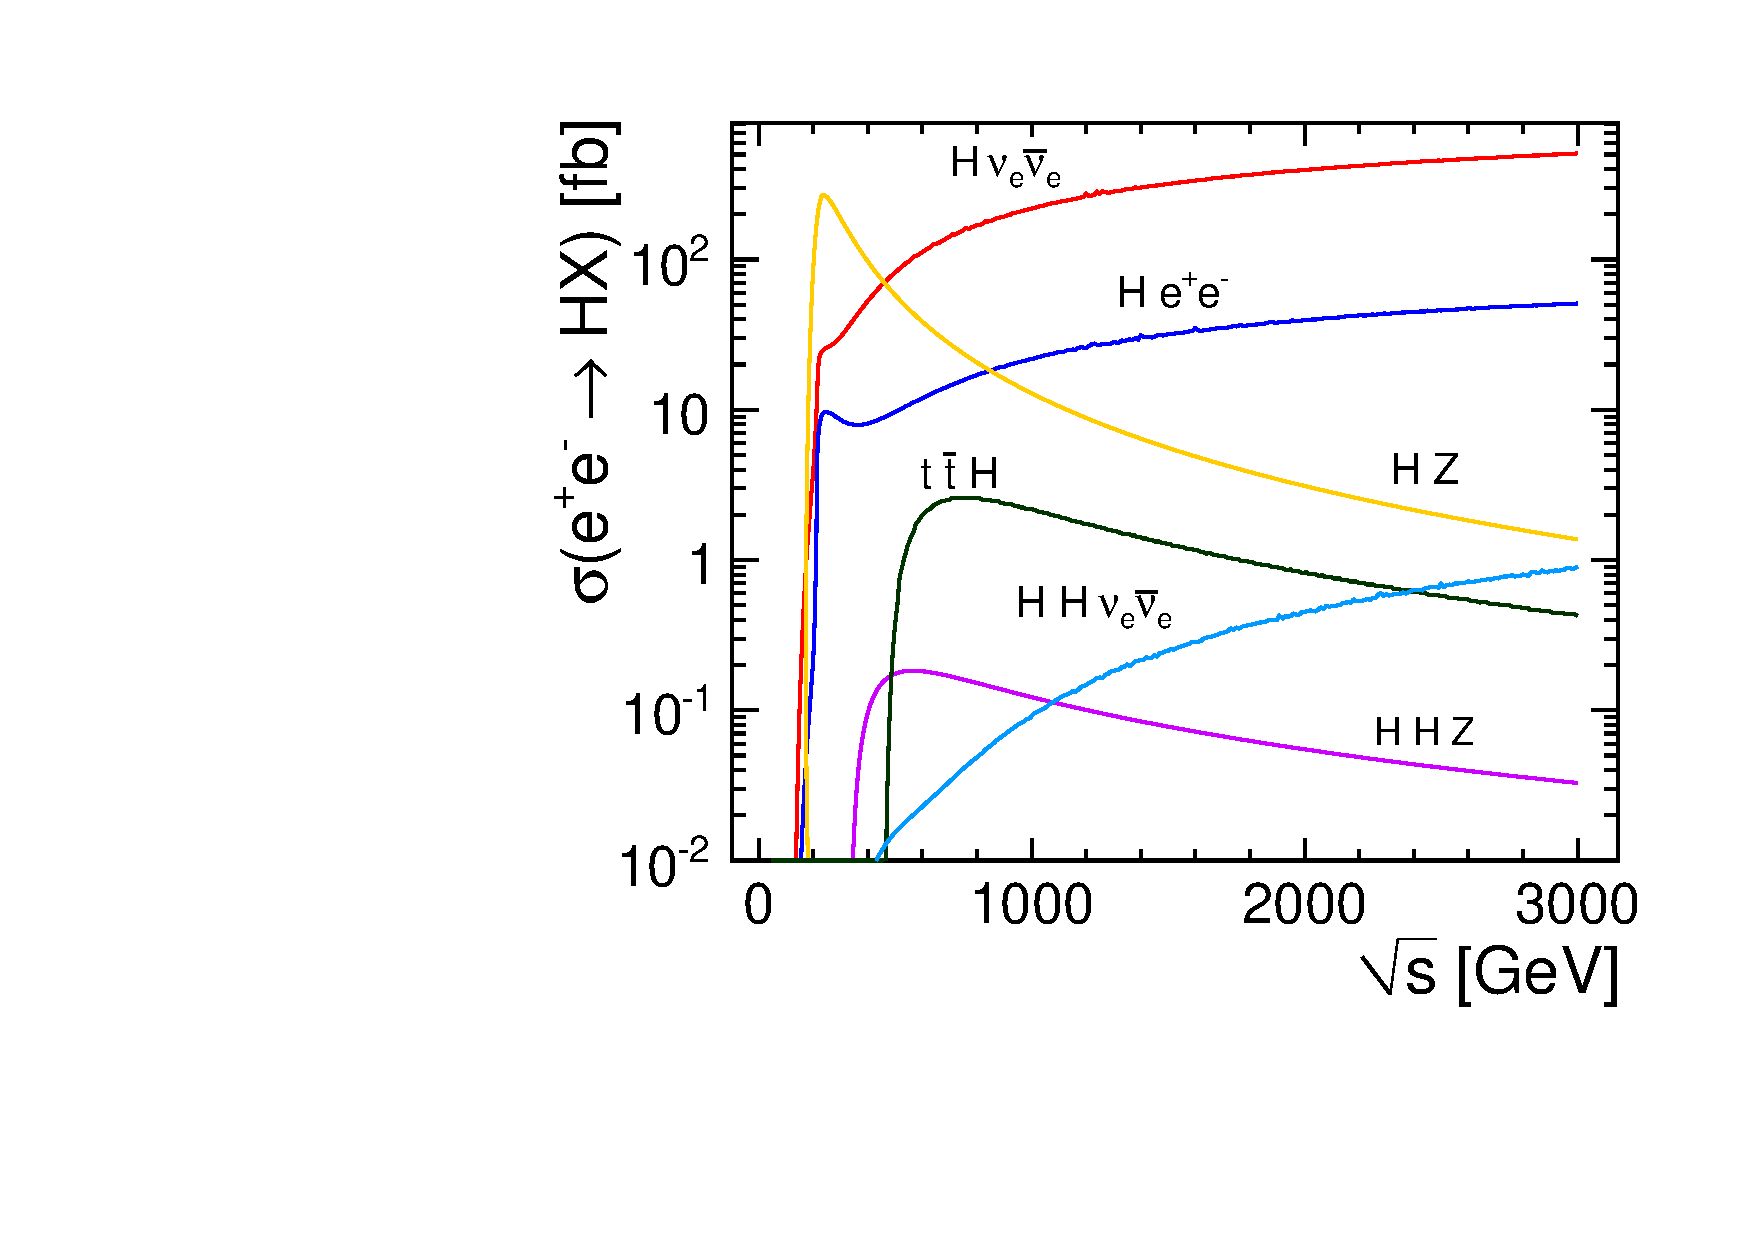
\includegraphics[width=4cm]{../SIDWorkshop/xsec_vs_cme.pdf}
\begin{tabular}{cc}
gHbb & 2\%\\
gHcc & 3\% \\
$gH\mu\mu$ & 15\%
\end{tabular}
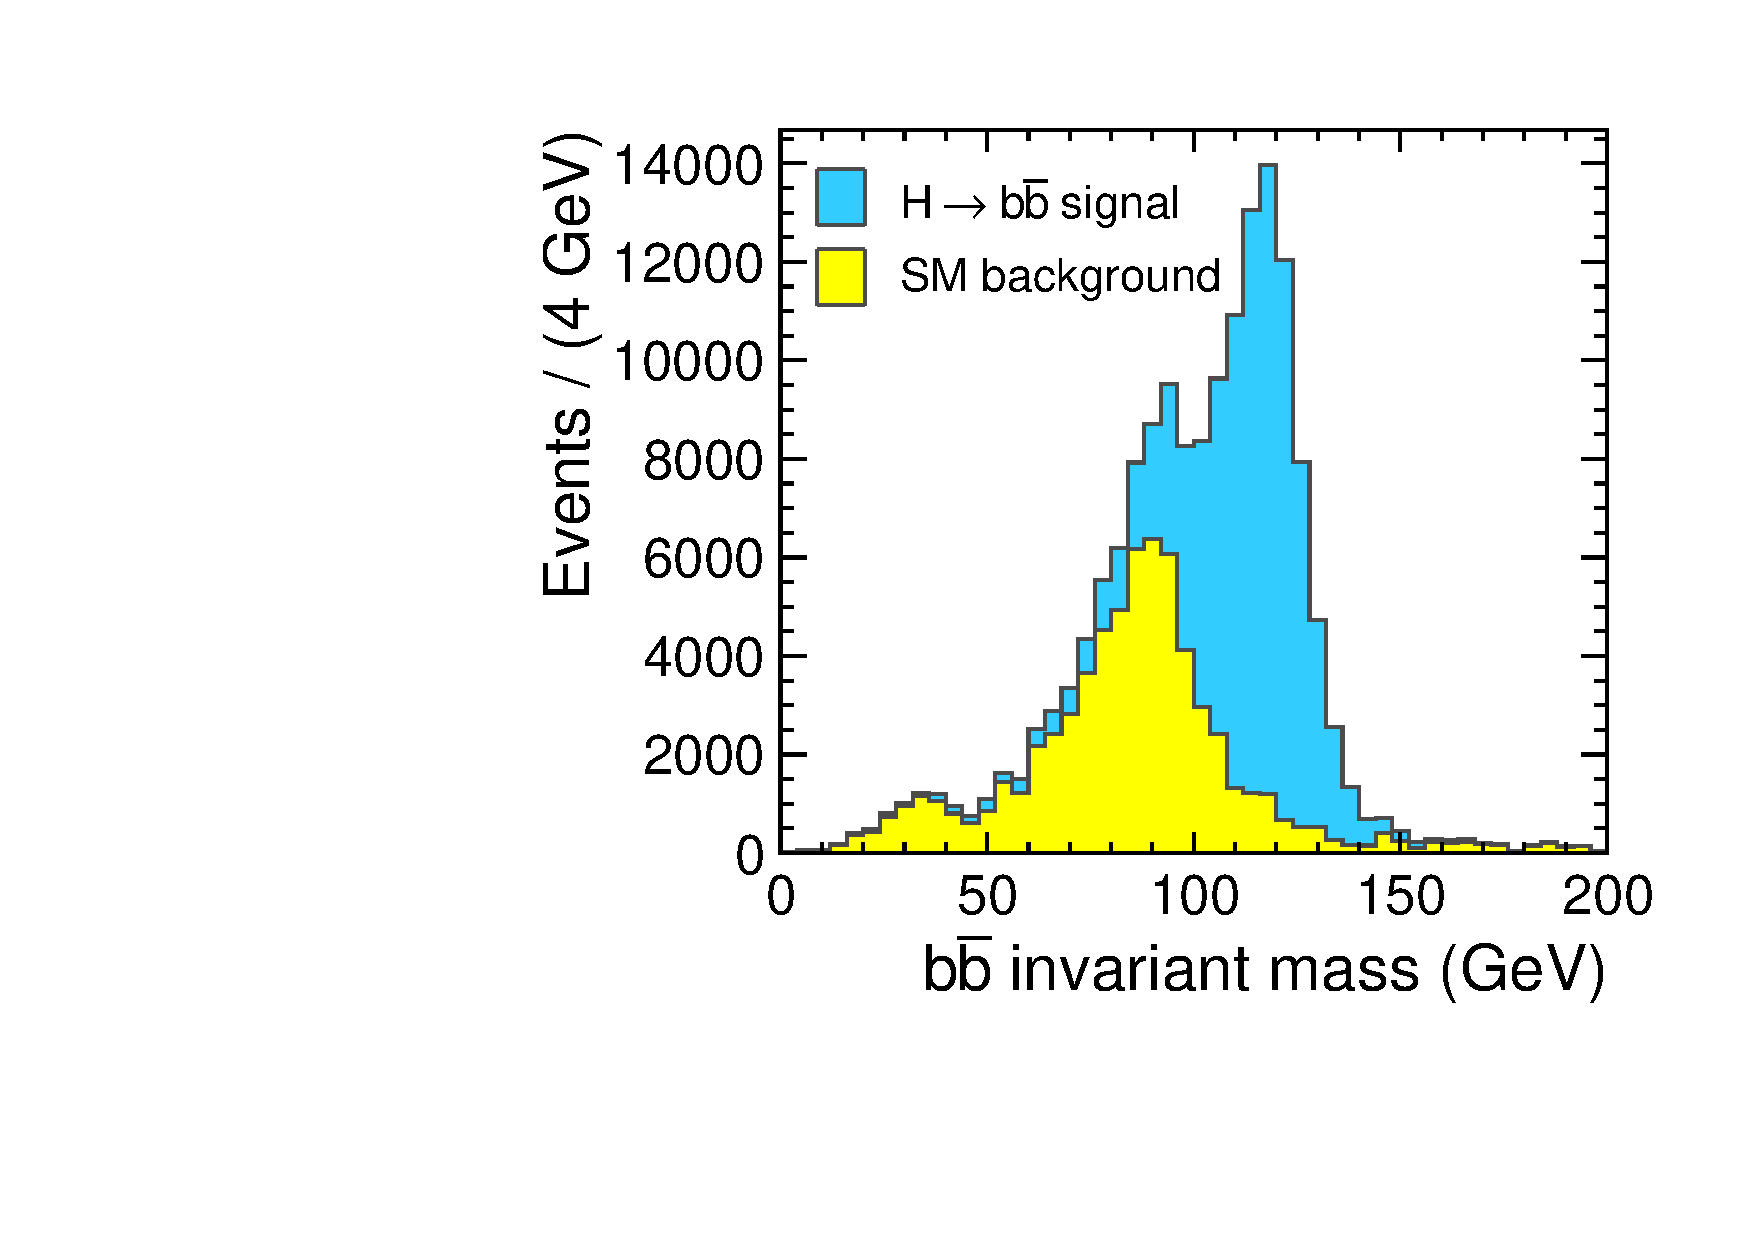
\includegraphics[width=4cm]{../SIDWorkshop/ee_h_bb_mass_mh120GeV.pdf}
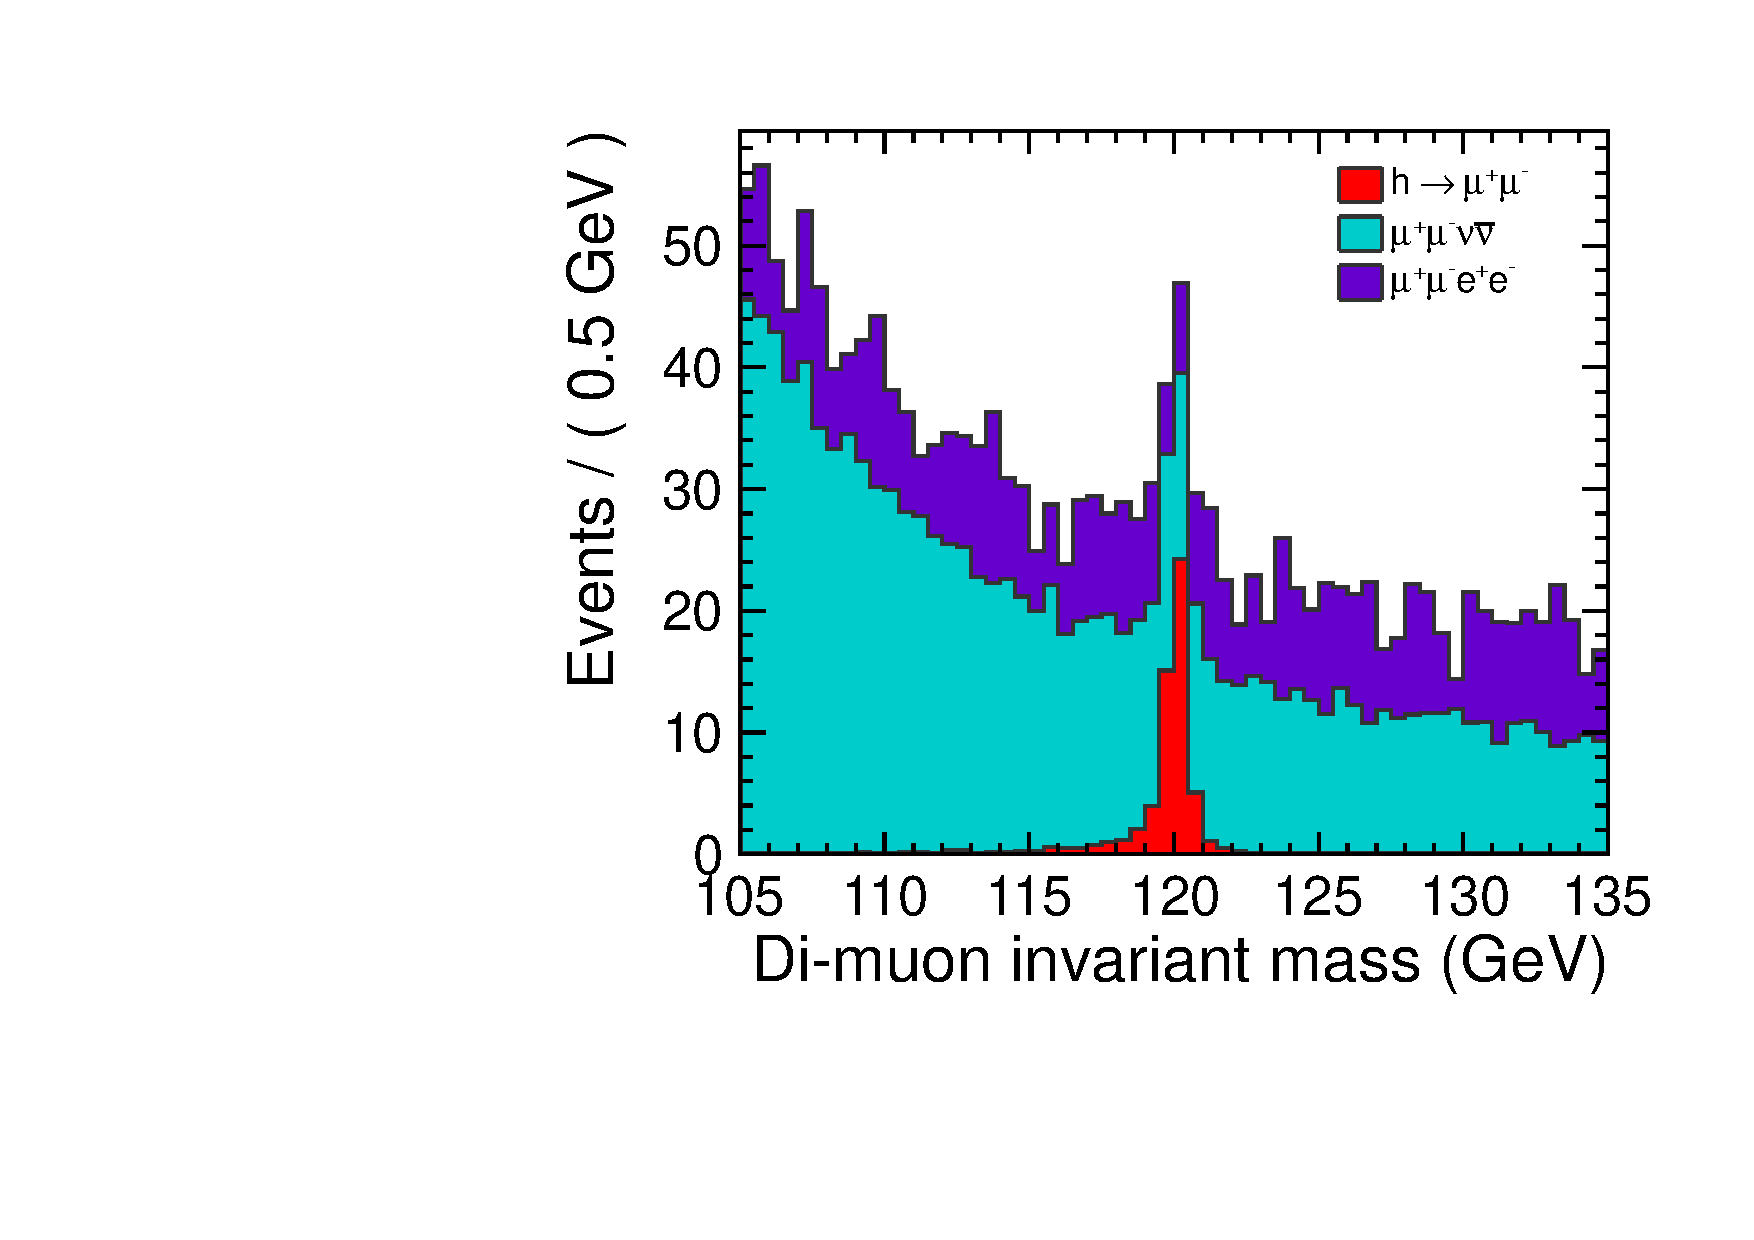
\includegraphics[width=4cm]{../SIDWorkshop/ee_h_mumu_mass_mh120GeV.pdf}
Ongoing studies for tri linear couplings $\lambda_{HHH}$.
\end{frame}
\begin{frame}
\frametitle{BSM Higgs}
Produced with $\Pep\Pem \to \PA+\Ph/\PH$, $\PA$ and $\PH$ are degenerate in
mass at studied point (tan b = 30, mA approx 750 GeV). $\PA\to bb$ and $\PH \to
bb$

$\Pep\Pem \to \PHp\PHm$, $\PHp\to tb$
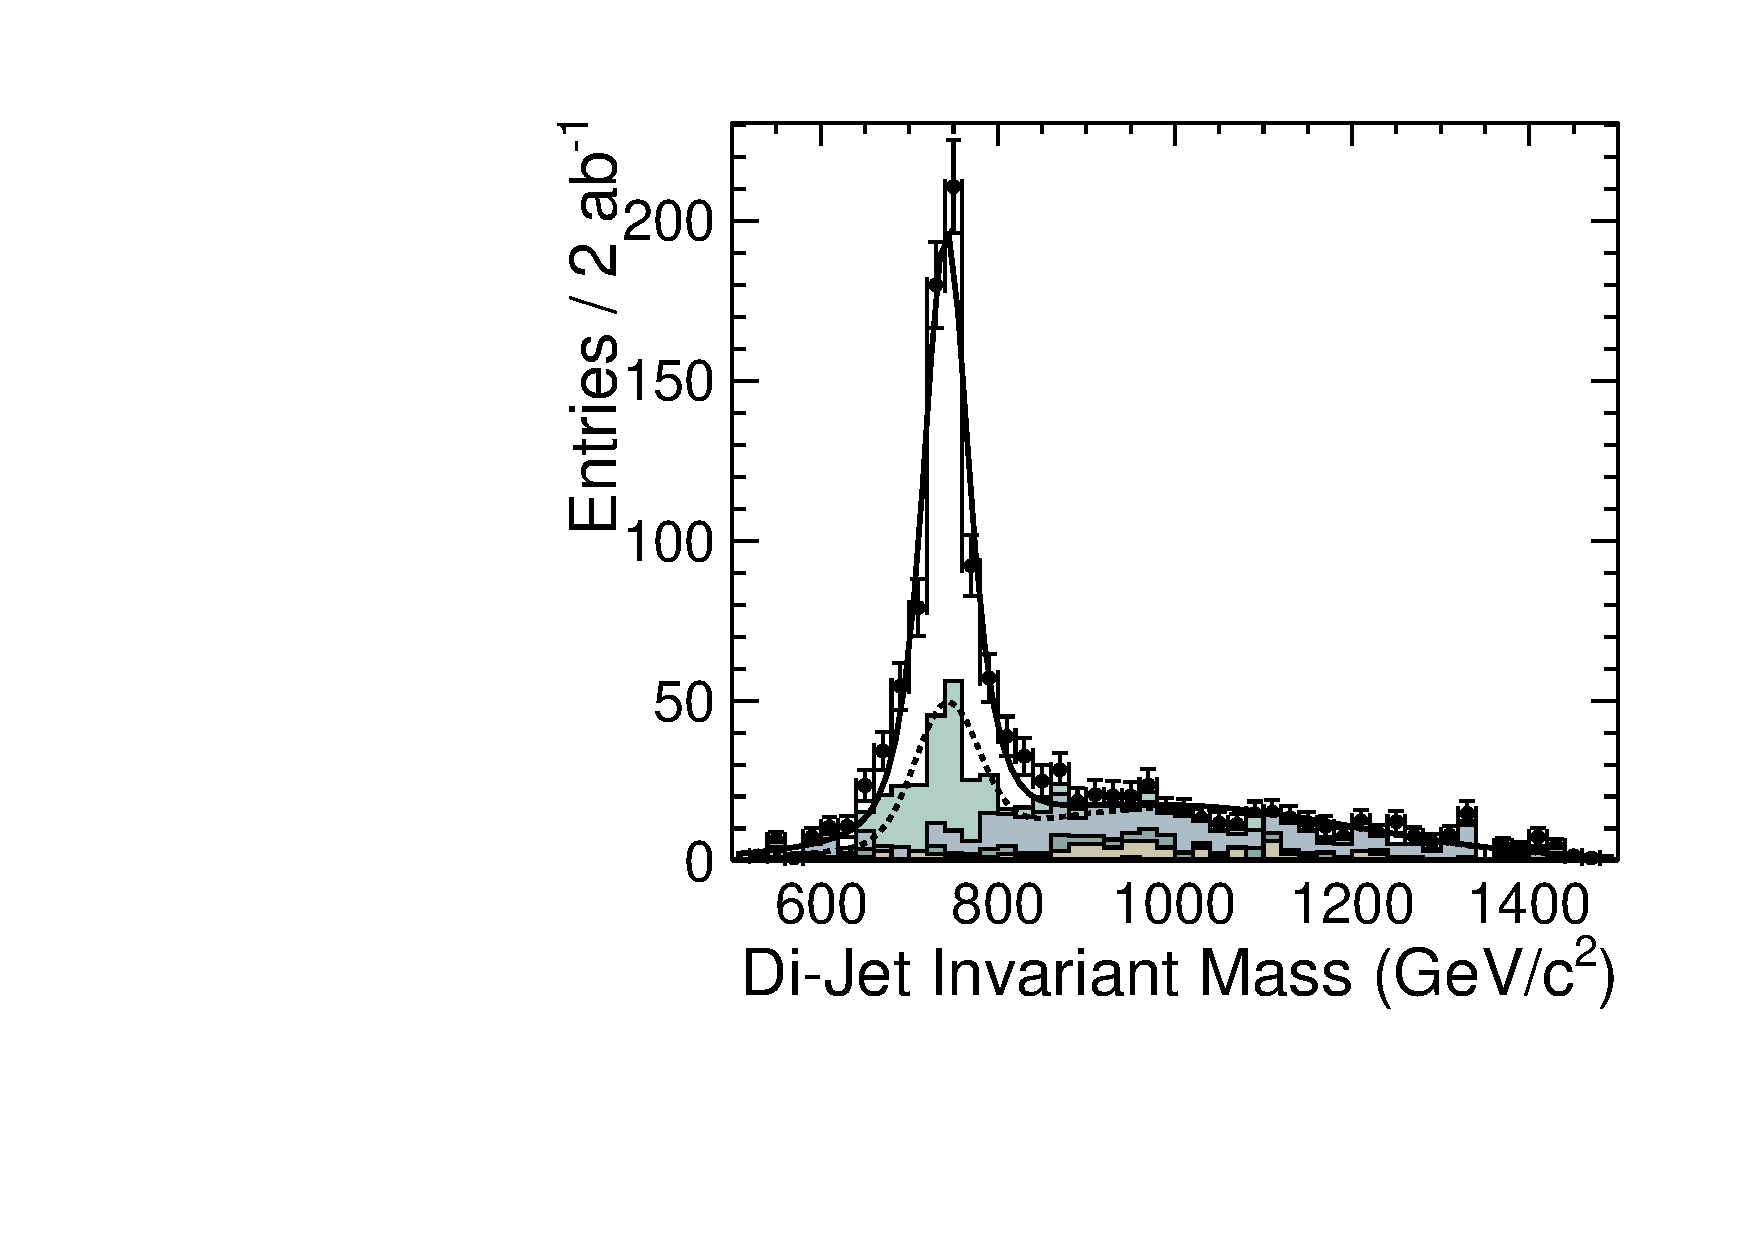
\includegraphics[width=5cm]{../SIDWorkshop/HAMass742_Bkg_CKFM_00BX_FJ.pdf}
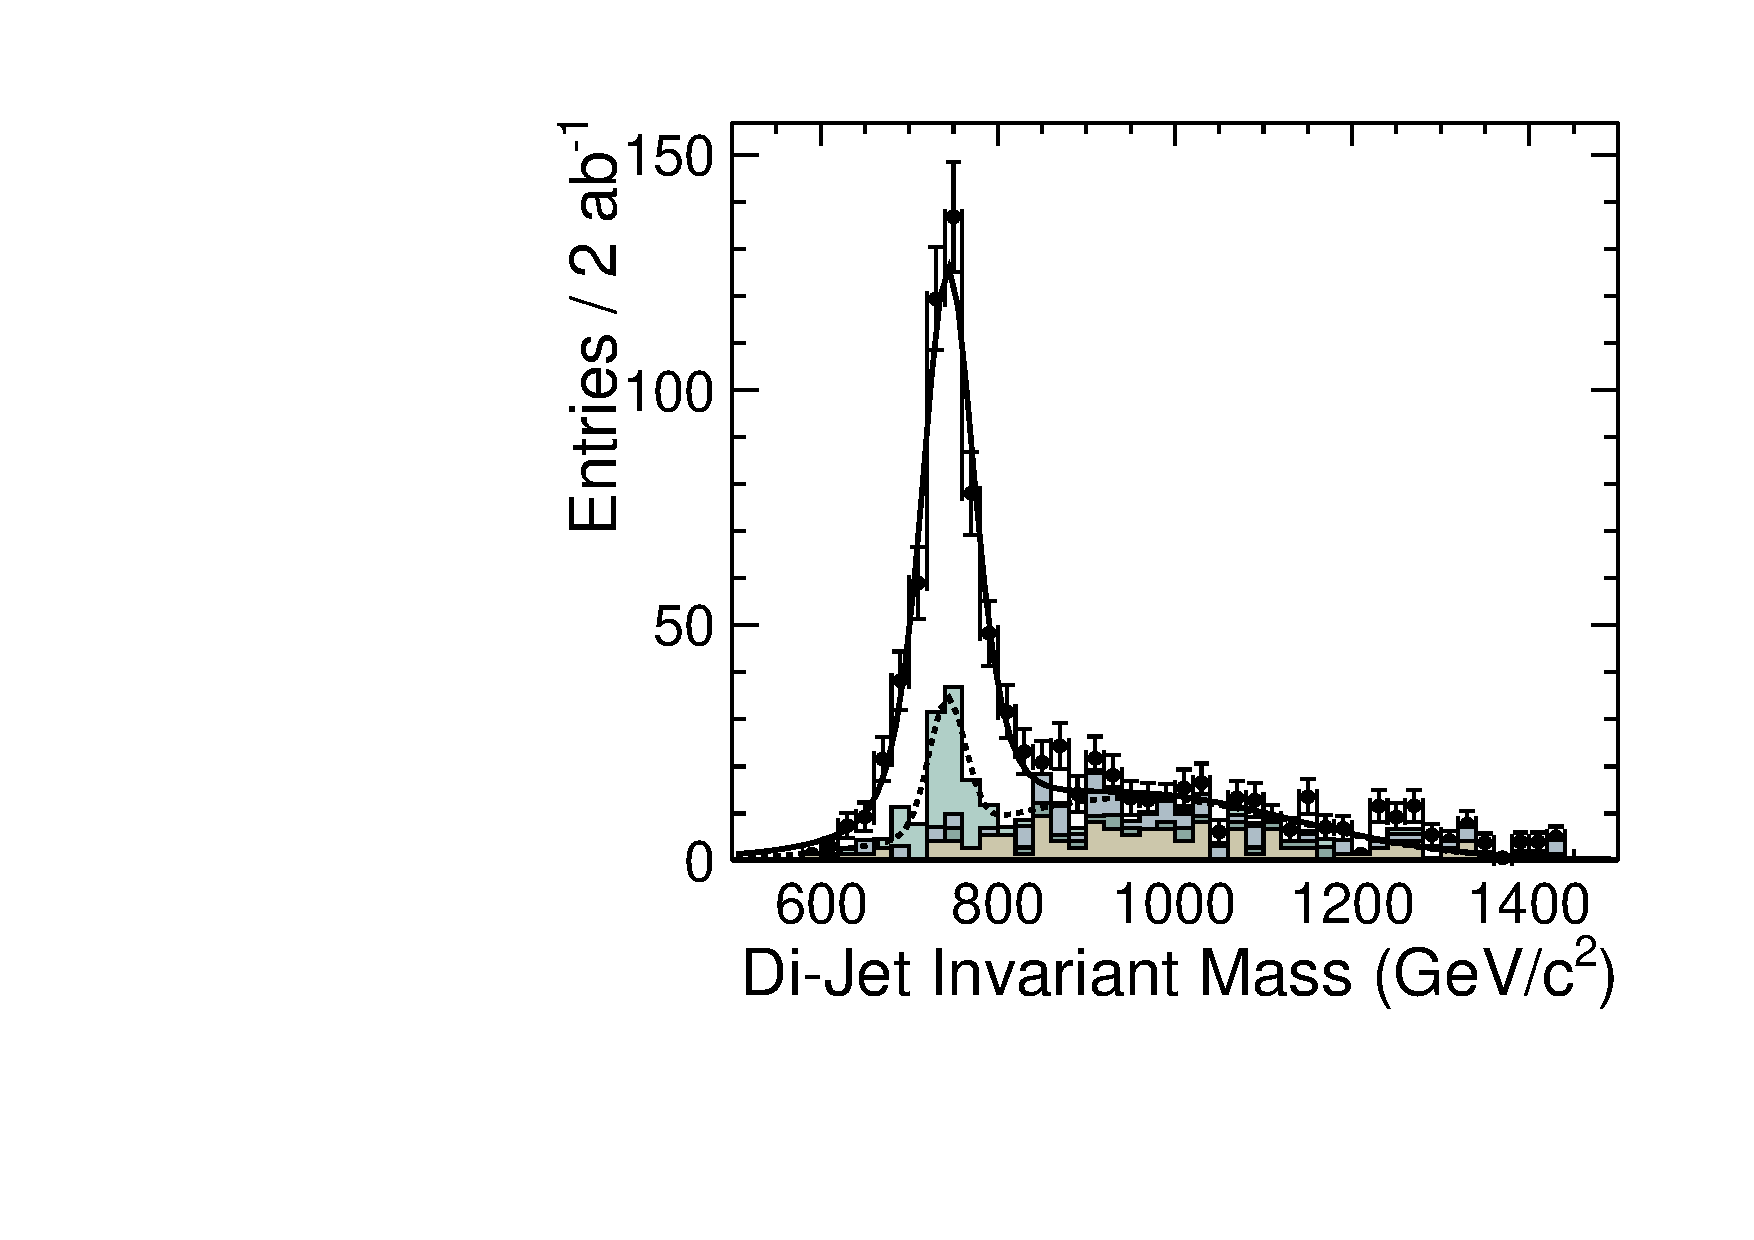
\includegraphics[width=5cm]{../SIDWorkshop/Hpm_Mass742_Bkg_CKFM_00BX_FJ.pdf}
\begin{tabular}{ccc}
\toprule
~ & mass & width\\
\midrule
A/H & 0.002 & 0.10\\
Hpm & 0.005 & 0.15\\
\bottomrule
\end{tabular}
relative deternmination of tan b $<$ 0.06
\end{frame}
\begin{frame}
\frametitle{SUSY}
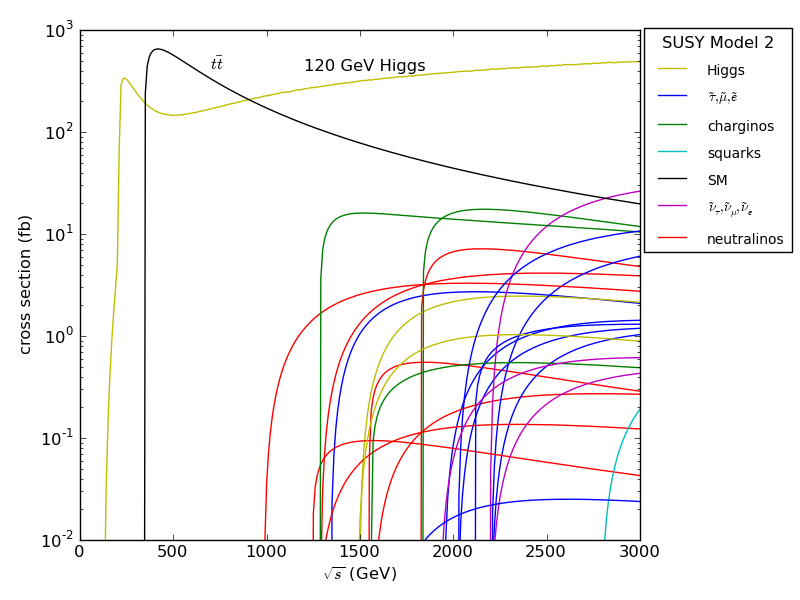
\includegraphics[width=5cm]{../SIDWorkshop/susy_model2.png}

Study chargino and neutralino masses by measuring kinematic endpoints of the
energy distributions, in channels like $neu2\to \Ph neu1$ Shown later in great
detail

Susy breaking models:
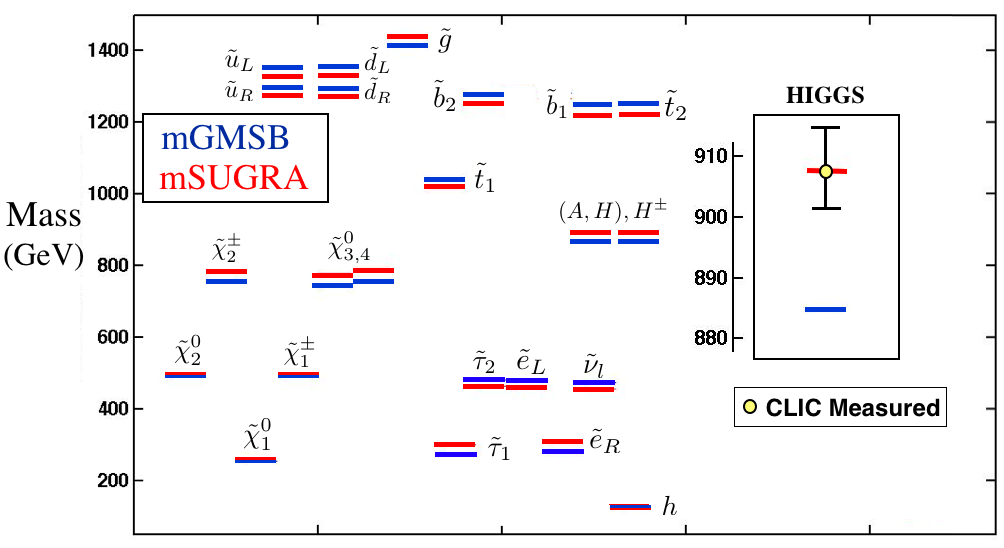
\includegraphics[width=5cm]{../SIDWorkshop/GvM.png}
\end{frame}
\begin{frame}
\frametitle{Other studies}
\begin{itemize}
  \item High scale stucture of SUSY
  \item Neutralino Dark Matter hypothesis
  \item Higgs strong interaction
  \item Z'
  \item Contact interaction
  \item Extra dimensions
  \item 
\end{itemize}
\end{frame}
\begin{frame}
\frametitle{Physics potential summary}
\begin{center}
{\scriptsize
 \begin{tabular}{ ccccc }
    \toprule
 Machine &     LHC14 & SLHC & LC800 & CLIC3\\
 Luminosity & $100\textrm{fb}^{-1}$ & $1\textrm{ab}^{-1}$&
 $500\textrm{fb}^{-1}$& $1\textrm{ab}^{-1}$\\
\midrule
squarks [TeV] &   2.5 & 3 & 0.4 & 1.5 \\
sleptons [TeV] &   0.3 & - & 0.4 & 1.5 \\ 
$\textrm{Z}'$ ({\tiny SM ~couplings}) [TeV]  &  5 & 7 & 8 & 20   \\ 
%\Zprime ({\tiny SM~couplings})  &     5& 6  & 8 & 22 \\
%$q*$      &    6.5 & 7.5 & 0.8 & 3 \\
%$l*$       &   3.4 & - & 0.8 & 3 \\
2 extra dims $M_D$ [TeV]  &    9 & 12 & 5-8.5 & 20-30 \\
%$W_L W_L$      &  3.4sig& >3.4sig& -& 70sig\\
TGC (95\%)  ({\tiny \rm $\lambda_{\gamma} $~coupling}) &   0.001& 0.0006& 0.0004& 0.0001 \\
$\mu$ contact scale [TeV] &  15& - & 20 & 60 \\
Higgs compos. scale [TeV] & 5-7 & 9-12 & 45 & 60\\
    \bottomrule
  \end{tabular}
  }
 \end{center}
 CLIC can 
 \begin{itemize}
   \item extend the \textit{discovery reach} of LHC,
   \item offer the opportunity of \textit{precise measurements} of masses and
 couplings.
 \end{itemize}
\end{frame}


\section[CLIC]{The CLIC Machine}
\begin{frame}
\frametitle{CLIC machine CDR}
\begin{itemize}
  \item Released later in 2012
  \item Presents the different technical aspects of a CLIC machine
  \item Details the machine properties
\end{itemize}
Here: overview of those properties
\end{frame}
\begin{frame}
\frametitle{Technology}
2 beam acceleration scheme: drive beam and main beam
\begin{itemize}
  \item Gradient 100 MV/m
  \item Energy: from few-hundred GeV upgradable in steps up to 3 TeV; R\&D has
  focused on 3 TeV
\end{itemize}
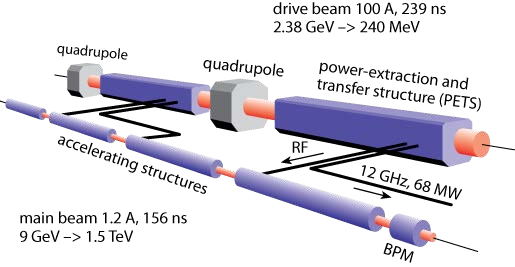
\includegraphics[width=5cm]{clicacceleration.png}
\end{frame}
\begin{frame}
\frametitle{Machine properties}
lumi, beam structure, compare to LHC/ILC, beam induced background
\begin{tabular}{ccc}
 & ILC 0.5TeV & CLIC 3TeV\\
 \hline
L [$\textrm{cm}^{-2}\,\textrm{s}^{-1}$] & $2\times 10^{34}$&$5.9\times 10^{34}$ \\
\hline
Bunch crossing separation  & 700 ns & 0.5 ns\\
\hline
Bunch crossings per train & 2670 & 312\\
\hline
Train repetition rate  & 5 Hz & 50 Hz\\
\hline
Crossing angle & 14mrad & 20mrad\\
\hline
\end{tabular}
\end{frame}
\begin{frame}
\frametitle{Machine Detector Interface}
Push-Pull system:\\
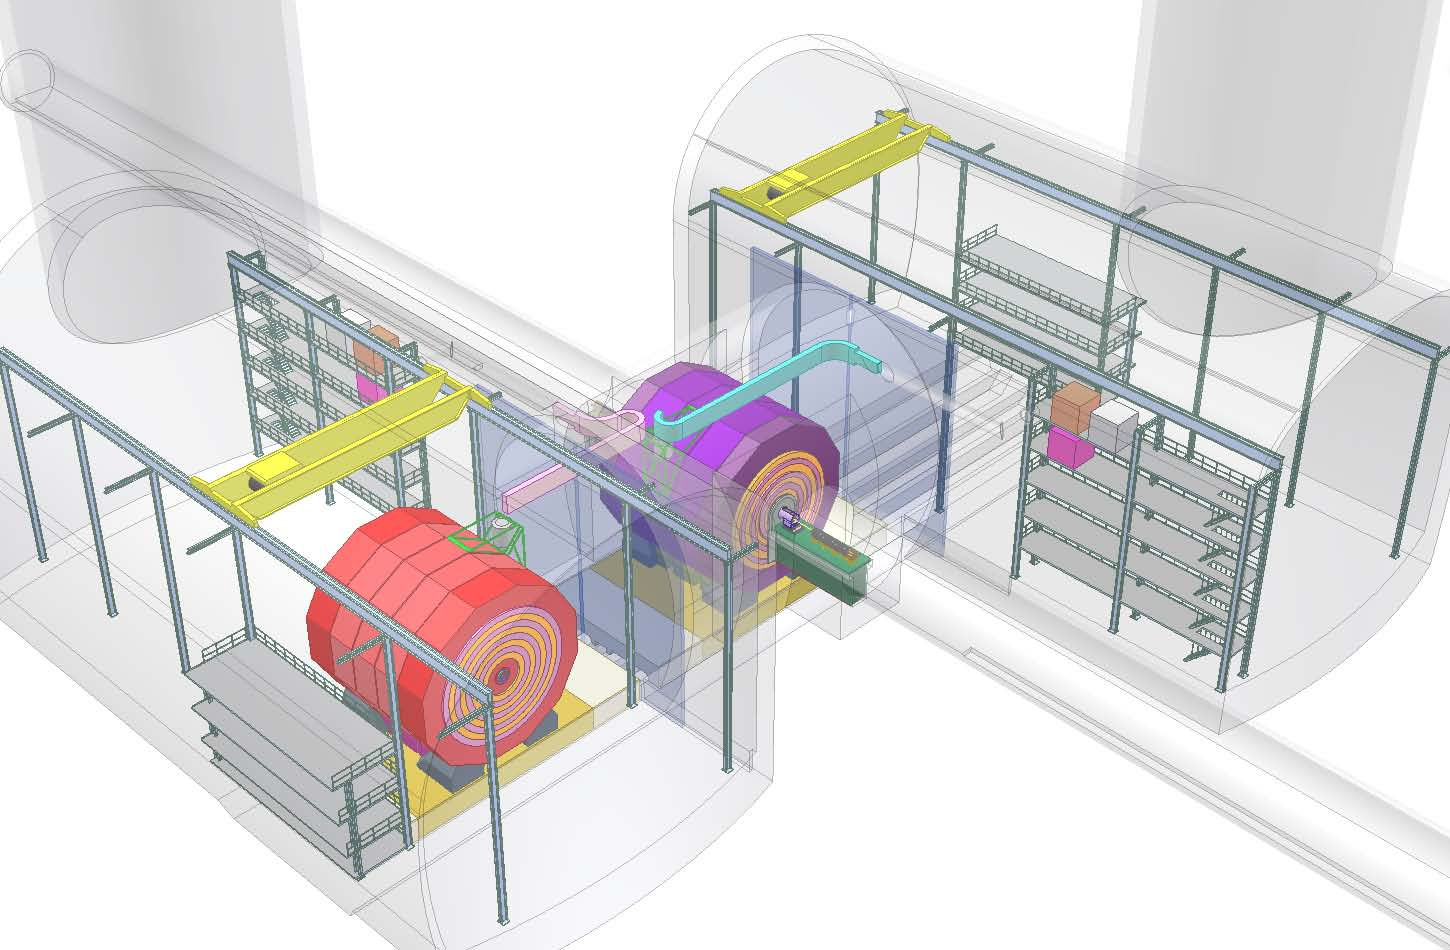
\includegraphics[width=10cm]{PushPull.png}
\end{frame}
\begin{frame}
\frametitle{Machine Detector Interface}
\includegraphics[width=10cm]{Figure_13_14.pdf}\\
Last accelerator element is IN the detector: alignment issue
\end{frame}

\begin{frame}
\frametitle{Machine induced backgrounds}
gg had, pairs, occupancy
\begin{tabular}{ccc}
 & ILC 0.5TeV & CLIC 3TeV\\
\hline
Nb $\gamma\gamma\to\textrm{had}$/BX & 0.2 & \alert{3.2}\\
\hline
Nb incoherant pairs/BX & $1\times 10^5$ & \alert{$3\times10^5$}\\
\hline
Nb coherent pairs/BX & $<10^2$ & $7\times 10^8$\\
\hline
\end{tabular}
\end{frame}

\section[Detectors]{The Detectors}
\begin{frame}
\frametitle{Required performance}
\begin{itemize}
  \item Trigger less readout of full train: time stamping, multi-hit capacity,
  filtering algorithms during reconstruction
  \item High resolution pixel detector for displaced vertices identification:\\
  {\scriptsize
  \begin{tabular}{lc}
  p = 1 Gev & $\sigma_{d0}\sim20\mu m$\\
  p = 100 GeV & $\sigma_{d0}\sim5\mu m$
  \end{tabular}
  }~\\ ~\\
  \item Momentum resolution:\\
  {\scriptsize 
  $\sigma(p_{\textrm{T}})/p_{\textrm{T}}^2\sim 10^{-5}\textrm{GeV}^{-1}$
   }~\\ ~\\
  \item Good jet-energy resolution (W/Z separation)\\
  {\scriptsize 
$\sigma(E_j)/E_j = 3.5\%-5\%$ for $E_j = 50\textrm{GeV}-1\textrm{TeV}$
  }~\\ ~\\
\end{itemize}
\end{frame}
\begin{frame}
\frametitle{Particle Flow}
\end{frame}
\begin{frame}
\frametitle{Overview}
\begin{columns}[c]
\column{6cm}
\centering
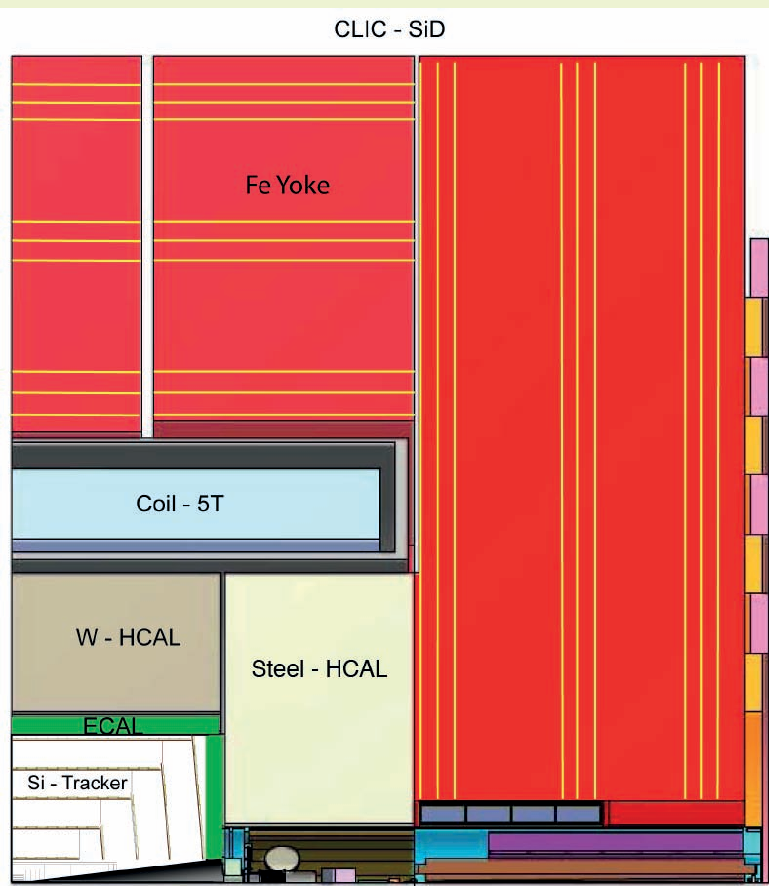
\includegraphics[width=5cm]{../SIDWorkshop/CLIC_SiD_xz.pdf}
\column{6cm}
\centering
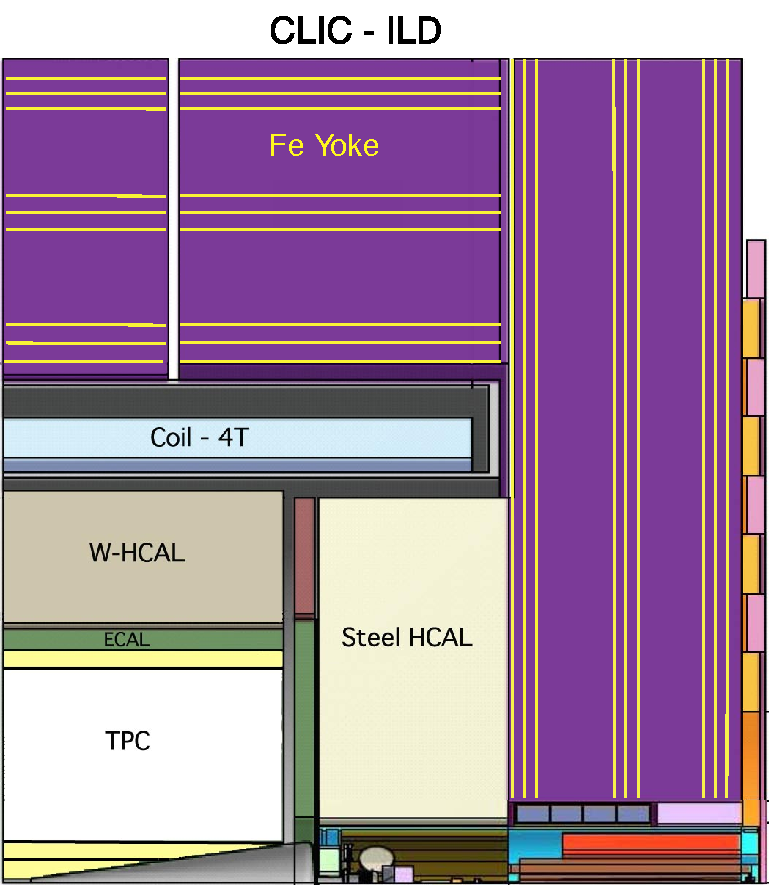
\includegraphics[width=5cm]{../SIDWorkshop/CLIC_ILD_xz.pdf}
\end{columns}
\end{frame}
\begin{frame}
\frametitle{Vertex detector optimization}
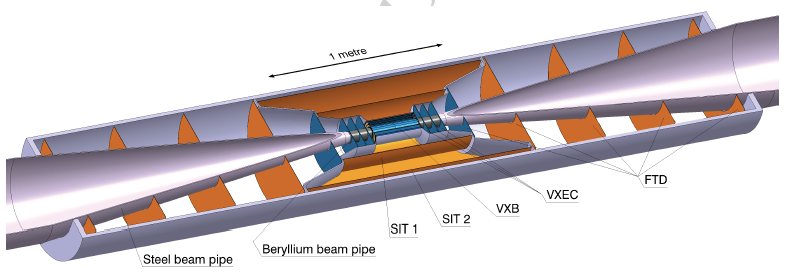
\includegraphics[width=8cm]{VertexDetector.png}
\begin{itemize}
  \item $20\times20\mu m$ pixel size
  \item 0.2\% X$_0$ material per layer (very thin)
  \item Time stamping 10ns
  \item Triggerless readout
  \item radiation level $<10^{11} n_{eq}cm^{-2}year^{-1}  \Leftarrow 10^4$ lower
  than LHC
\end{itemize}
\alert{Challenging R\&D project}
\end{frame}

\begin{frame}
\frametitle{Tracking in SiD}
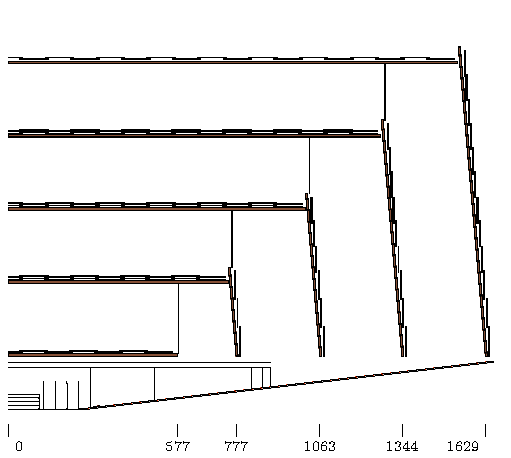
\includegraphics[width=5cm]{sid_tracker_zx.pdf}
\end{frame}
\begin{frame}
\frametitle{Tracking in ILD}
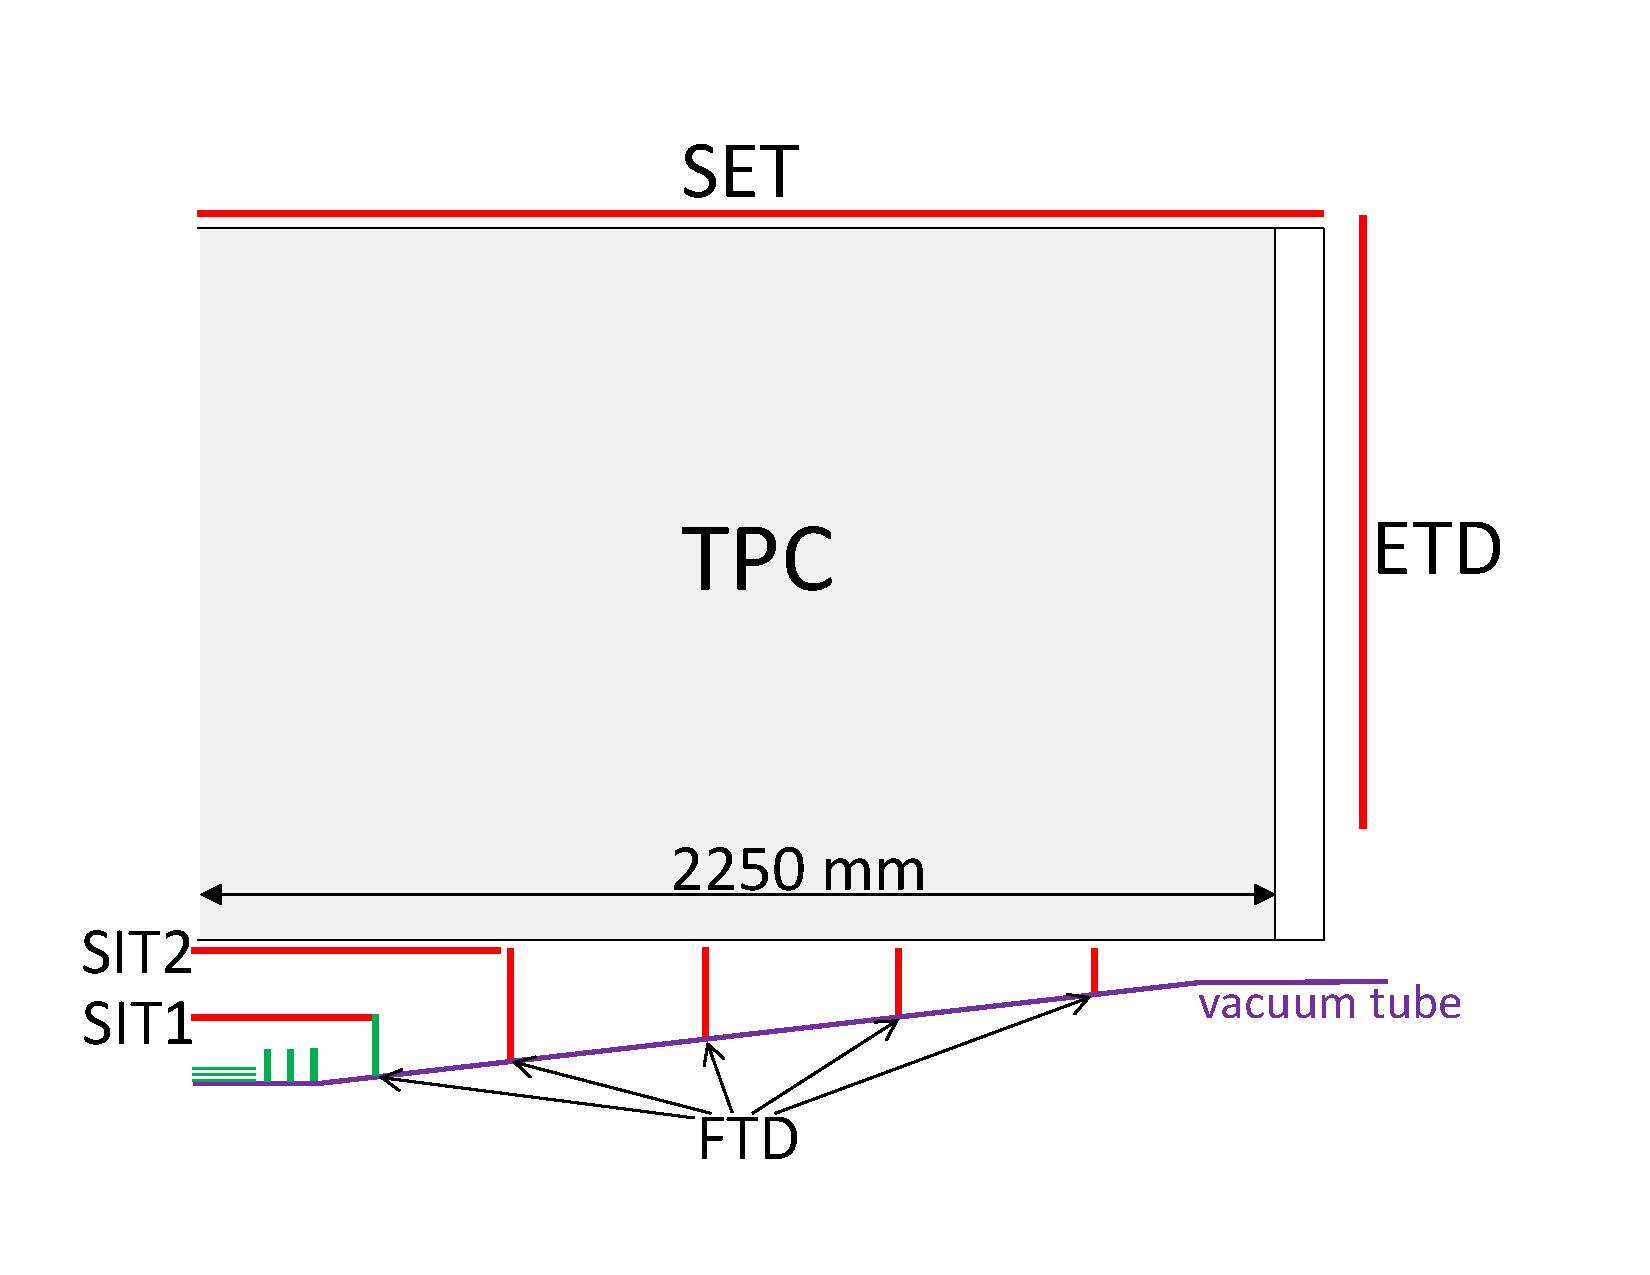
\includegraphics[width=5cm]{CLIC_ILD_tracking_geom.pdf}
\end{frame}
\begin{frame}
\frametitle{ECAL}
Use tungsten Fine grained for Particle Flow
\end{frame}
\begin{frame}
\frametitle{HCAL}
Use tungsten for lower depth
\end{frame}
\begin{frame}
\frametitle{CALICE results}
\end{frame}

\section[Bkg treatment]{Dealing with the machine induced background}
\begin{frame}
\frametitle{Timing cuts}
\end{frame}
\begin{frame}
\frametitle{Jet reconstruction}
\end{frame}

\section{Physics Results}
\begin{frame}
 \frametitle{Benchmark channels}
\end{frame}
\begin{frame}
\frametitle{SM Higgs}
\end{frame}
\begin{frame}
\frametitle{SM Higgs}
\end{frame}
\begin{frame}
\frametitle{Squarks}
\end{frame}
\begin{frame}
\frametitle{Squarks}
\end{frame}
\begin{frame}
\frametitle{Sleptons}
\end{frame}
\begin{frame}
\frametitle{Sleptons}
\end{frame}
\begin{frame}
\frametitle{Gauginos}
\end{frame}
\begin{frame}
\frametitle{Gauginos}
\end{frame}
\begin{frame}
\frametitle{Heavy Higgs}
\end{frame}
\begin{frame}
\frametitle{Top physics at 500GeV: vertex detector}
\end{frame}
\begin{frame}
\frametitle{Top physics at 500 GeV: compare with ILC}
\end{frame}

\section{Conclusion}
\begin{frame}
\frametitle{Overview}
\begin{itemize}
  \item Introduced the CLIC machine
  \item Presented the CLIC detectors concept
  \item Shown that it's possible to deal with the machine induced background
  \item High precision physics possible
\end{itemize}
\end{frame}
\begin{frame}
\frametitle{Signatory list}
\textit{You are cordially invited to subscribe to the CDR Signatories List:\\
\begin{itemize}
\item If you have made contributions to the CLIC accelerator or the Linear
Colliders Physics and Detector studies, or intend to contribute in the future,
\end{itemize}
~\\
OR / AND\\
~\\
\begin{itemize}
  \item If you wish to express support to the physics case and the study of a
  multi-TeV Linear Collider based on the CLIC technology, and its detector
  concepts.
\end{itemize}
}
\url{https://indico.cern.ch/conferenceDisplay.py?confId=136364}
\end{frame}

\appendix

\section{Software}
\begin{frame}
\frametitle{Generation}
\end{frame}
\begin{frame}
\frametitle{Simulation}
\end{frame}
\begin{frame}
\frametitle{Handling background in the software}
\end{frame}
\begin{frame}
\frametitle{Reconstruction}
\end{frame}
\begin{frame}
\frametitle{Using the GRID: ILCDIRAC}
\end{frame}

\end{document}